\newpage
\subsection{Caso d'uso UC13: Ricerca utente}
\label{UC11}
\begin{figure}[h]
	\centering
	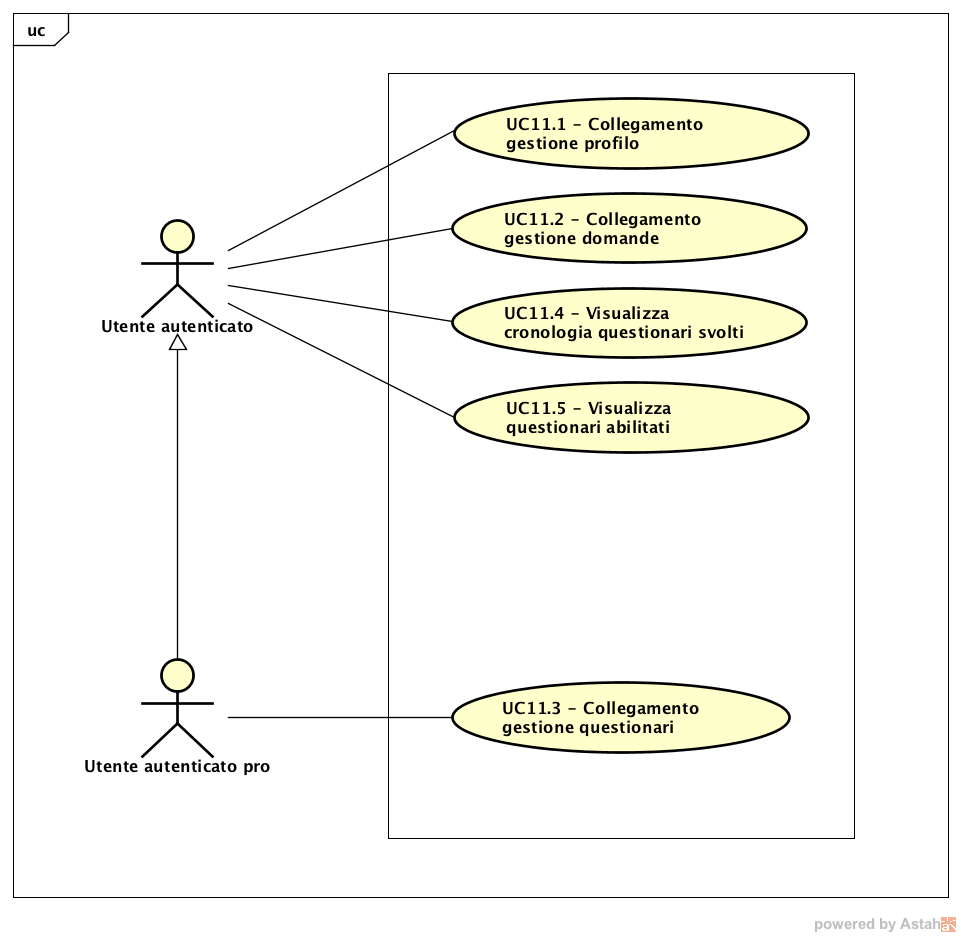
\includegraphics[scale=0.5]{UML/UC11.png}
	\caption{UC13: Ricerca utente}
\end{figure}
\FloatBarrier
\begin{itemize}
	\item \textbf{Attori}: utente autenticato, utente autenticato pro;
	\item \textbf{Descrizione}: l'attore può ricercare un utente registrato al sistema;
	\item \textbf{Precondizione}: il sistema visualizza la barra di ricerca per gli utenti registrati;
	\item \textbf{Postcondizione}: il sistema visualizza il profilo utente dell' utente ricercato;
	\item \textbf{Scenario principale}:
	\begin{enumerate}
		\item L'attore può inserire nome e cognome/username dell'utente che vuole ricercare (UC5.1);
		\item L'attore può selezionare l'utente ricercato per visualizzarne il profilo (UC5.2).
	\end{enumerate} 
	\item \textbf{Estensione}: la ricerca dell'utente è fallita (UC5.3);
	\item \textbf{Scenario alternativo}: l'utente ha inserito nella barra di ricerca un nome e cognome/username inesistente all'interno del sistema. 
\end{itemize}

\subsubsection{Caso d'uso UC13.1: Inserimento nome e cognome/usermane}

\begin{itemize}
	\item \textbf{Attori}: utente autenticato, utente autenticato pro;
	\item \textbf{Descrizione}: l'attore può inserire nome e cognome/username di un utente nella barra di ricerca;
	\item \textbf{Precondizione}: il sistema visualizza la barra di ricerca degli utenti;
	\item \textbf{Postcondizione}: l'attore ha inserito nome e cognome/username dell'utente che vuole ricercare;
	\item \textbf{Scenario principale}: l'attore inserisce il nome e cognome/username dell'utente che vuole ricercare.
\end{itemize}

\subsubsection{Caso d'uso UC13.2: Selezione utente ricercato}

\begin{itemize}
	\item \textbf{Attori}: utente autenticato, utente autenticato pro;
	\item \textbf{Descrizione}: l'attore può selezionare l'utente ricercato per visualizzarne il profilo;
	\item \textbf{Precondizione}: l'utente ha inserito il nome e congome/username dell'utente ricercato nella barra di ricerca e la ricerca è andata a buon fine;
	\item \textbf{Postcondizione}: il sistema visualizza il profilo dell'utente selezionato;
	\item \textbf{Scenario principale}: l'attore seleziona l'utente ricercato per visualizzarne il profilo.
\end{itemize}

\subsubsection{Caso d'uso UC13.3: Ricerca utente fallita}

\begin{itemize}
	\item \textbf{Attori}: utente autenticato, utente autenticato pro;
	\item \textbf{Descrizione}: il sistema mostra un messaggio di fallimento della ricerca poichè l'attore ha inserito nome e cognome/username di un utente inesistente;
	\item \textbf{Precondizione}: l'attore ha inserito nome e cognome/username di un utente inesistente;
	\item \textbf{Postcondizione}: il sistema mostra un messaggio di fallimento della ricerca;
	\item \textbf{Scenario principale}: il sistema mostra un messaggio di fallimento della ricerca dell'utente.
\end{itemize}